\documentclass[aspectratio=169,10pt]{beamer}
\usepackage[utf8]{inputenc}
\usepackage[T1]{fontenc}
\usepackage[spanish]{babel}
\usepackage{booktabs}
\usepackage{graphicx}
\usepackage{array}
\definecolor{ok}{RGB}{25,125,70}
\definecolor{warn}{RGB}{190,125,15}
\definecolor{stop}{RGB}{180,45,45}
\setbeamertemplate{navigation symbols}{}
\setbeamertemplate{footline}{\hfill\insertframenumber\hspace{1em}\vspace{0.6em}}
\newcommand{\source}[1]{\vfill{\tiny\color{gray}Fuente: #1}}
\newcommand{\upcode}{análisis upstream ATLAS-SUSY-2018-13 (congelado)}
\newcommand{\validated}{\textcolor{ok}{\textbf{VALIDATED}}}
\newcommand{\blocked}{\textcolor{stop}{\textbf{BLOCKED}}}
\begin{document}

\begin{frame}{Un escalar de larga vida puede decaer dentro del tracker}
  {\Large\textbf{Recast DV+jets: estado reproducible}}\par\vspace{0.25em}
  {\large Camino hacia la reinterpretación DiHiggs/2HDM\hfill\normalsize 15-07-2026}\par
  \vspace{0.9em}
  \begin{columns}[T]
    \column{0.46\textwidth}
    \textbf{Señal}: $gg\to h^*\to SS$, con $S$ de larga vida.
    \begin{itemize}
      \item Si $S$ decae dentro del tracker, sus productos cargados
            pueden formar un vértice desplazado (DV).
      \item La escala del desplazamiento es $\beta\gamma c\tau$.
    \end{itemize}
    \column{0.46\textwidth}
    \textbf{Selección}: un DV multitrack junto a jets.
    \begin{itemize}
      \item Los jets dan el trigger y las regiones de señal.
      \item La eficiencia depende del boost, la vida media y la topología.
    \end{itemize}
  \end{columns}
  \source{plan de reproducción; contrato físico de scalar-recast-v0}
\end{frame}

\begin{frame}{Compilar el análisis no equivale a reproducir su física}
  \begin{columns}[T]
    \column{0.46\textwidth}
    \textbf{Un recast es}
    \begin{itemize}
      \item una implementación aproximada de una selección publicada;
      \item una cadena que se valida contra un benchmark conocido;
      \item una medida de aceptación $\times$ eficiencia, separada de la tasa.
    \end{itemize}
    \column{0.46\textwidth}
    \textbf{Un recast no es}
    \begin{itemize}
      \item una simulación completa de ATLAS;
      \item física validada por el hecho de compilar;
      \item algo que un factor $K$ pueda arreglar.
    \end{itemize}
  \end{columns}
  \vspace{0.9em}
  \centering
  La normalización mueve la escala; no mueve eventos entre cortes.
  \source{contrato de validación}
\end{frame}

\begin{frame}{El DV se reconstruye con tracks, no con jets}
  \begin{columns}[T]
    \column{0.40\textwidth}
    \centering
    \vspace{0.6em}
    $\vec x_{\rm dec}\ \longrightarrow\ R_{xy}$\\[0.9em]
    tracks del decaimiento\\[0.6em]
    $\longrightarrow\ |d_0|>2$ mm
    \column{0.56\textwidth}
    El análisis parte de la posición de decaimiento y exige:
    \begin{enumerate}
      \item decaimiento en la región fiducial, con $R_{xy}>4$ mm;
      \item al menos un track con $|d_0|>2$ mm;
      \item $\geq5$ productos cargados seleccionados;
      \item $m_{DV}>10$ GeV.
    \end{enumerate}
  \end{columns}
  \vspace{0.7em}
  Dónde cae el vértice lo deciden el boost y la vida media: la escala es $\beta\gamma c\tau$.
  \source{\upcode}
\end{frame}

\begin{frame}{Los jets seleccionan el evento; los tracks forman el DV}
  \begin{itemize}
    \item \textbf{Trigger}: sin jets el evento no se registra.
    \item \textbf{ISR}: puede ser decisivo cuando la producción escalar deja poca
          actividad hadrónica propia.
    \item \textbf{Decaimiento del LLP}: $b\bar b$, $gg$ y bosones hadrónicos aportan jets.
    \item \textbf{Pero un jet no prueba desplazamiento}: el DV sale de la posición
          del decaimiento y de los tracks, no del jet.
  \end{itemize}
  \vspace{0.9em}
  \centering\textbf{Los jets hacen visible el evento; el DV lo demuestran los tracks.}
  \source{\upcode}
\end{frame}

\begin{frame}{Gate B valida la cadena completa, no el ejecutable}
  \vspace{0.5em}
  \centering\large
  \fbox{MadGraph}\ $\rightarrow$ \fbox{LHE}\ $\rightarrow$ \fbox{Pythia 8}\\[1em]
  $\rightarrow$ \fbox{FastJet / toy detector}\ $\rightarrow$ \fbox{DV}\ $\rightarrow$ \fbox{cutflow}
  \vspace{1.2em}

  \normalsize\raggedright
  Cada interfaz aporta su propia forma de fallar: proceso y merging en MadGraph,
  shower y decaimientos en Pythia, jets y eficiencias en el detector de juguete.
  Por eso cada una necesita cards, versiones, seeds y checksums en un manifest.
  \source{contrato de validación; plan de reproducción}
\end{frame}

\begin{frame}{Por qué usamos primero la referencia SUSY}
  \begin{columns}[T]
    \column{0.48\textwidth}
    \textbf{strong-bm1, la muestra distribuida}
    \begin{itemize}
      \item $pp\to\tilde g\tilde g$ + 0/1/2 partones;
      \item 10.000 eventos por multiplicidad;
      \item masas 2000/850 GeV;
      \item merging CKKW--L a 500 GeV.
    \end{itemize}
    \column{0.48\textwidth}
    \textbf{El neutralino no es nuestro modelo}
    \begin{itemize}
      \item pertenece únicamente a la línea base SUSY;
      \item el código lo fija por PDG hardcoded;
      \item tras Gate B, $S$ ocupa ese lugar.
    \end{itemize}
  \end{columns}
  \vspace{0.9em}
  \centering
  Sin línea base no sabríamos si un desacuerdo viene de la generación,
  del shower o de nuestra adaptación.
  \source{contrato strong-bm1; \upcode}
\end{frame}

\begin{frame}{Qué está listo y qué sigue bloqueado}
  \vspace{0.3em}
  \begin{tabular}{p{0.62\textwidth}l}
    \toprule
    Stack de software (Pythia/FastJet/MadGraph) & \textcolor{ok}{\textbf{PASS}}\\
    Parche A/B + build upstream & \textcolor{ok}{\textbf{PASS}}\\
    Selección de jets A/B (toy) & \textcolor{ok}{\textbf{PASS}}\\
    Propagación de vida del LLP & \textcolor{stop}{\textbf{FAIL}}\\
    Eficiencia DV & \textcolor{warn}{\textbf{NOT EVALUATED}}\\
    Ejecutable MadGraph & \textcolor{ok}{\textbf{AVAILABLE}}\\
    UFO físico (2HDM) & \textcolor{stop}{\textbf{MISSING}}\\
    \bottomrule
  \end{tabular}
  \vspace{0.9em}

  Pythia, FastJet y MadGraph 3.5.3 ya están instalados; el único bloqueo de MadGraph
  para producción física es el UFO. La bifurcación A/B funciona, pero todo decae
  como si fuera prompt: Gate B sobre strong-bm1 sigue \blocked.
  \source{M1 build report; M2 strong-bm1 contract report; Mission 01 execution report}
\end{frame}

\begin{frame}{La bifurcación A/B funciona; el transporte LLP aún no}
  \begin{columns}[T]
    \column{0.46\textwidth}
    \textbf{Selección trackless} (toy $m=250$ GeV, $c\tau=5.1$ mm)
    \begin{itemize}
      \item Original: 25.0\%
      \item Modificada: \textbf{51.6\%}
    \end{itemize}
    {\small Mismo LHE/SLHA; cambio atribuible sólo a la estrategia de selección.}
    \column{0.46\textwidth}
    \textbf{Tres resultados, no uno}
    \begin{enumerate}
      \item la infraestructura compila y ejecuta;
      \item la bifurcación A/B de jets funciona;
      \item el vértice desplazado \textbf{no} está validado.
    \end{enumerate}
  \end{columns}
  \vspace{0.7em}
  \centering
  \textcolor{stop}{\textbf{Las etapas DV permanecen en cero: fallo de propagación de vida en Pythia.}}
  \par\vspace{0.4em}
  \raggedright\tiny\texttt{AB\_JET\_SELECTION\_UNIT\_TEST} \quad \texttt{DV\_LIFETIME\_PLUMBING\_FAILED} \quad \texttt{PAPER\_TABLE\_PROXY\_NOT\_EXCLUSION}
  \source{Mission 01 execution report; package/results/ab\_summary.md}
\end{frame}

\begin{frame}{El objetivo numérico que Gate B tendrá que igualar}
  \centering
  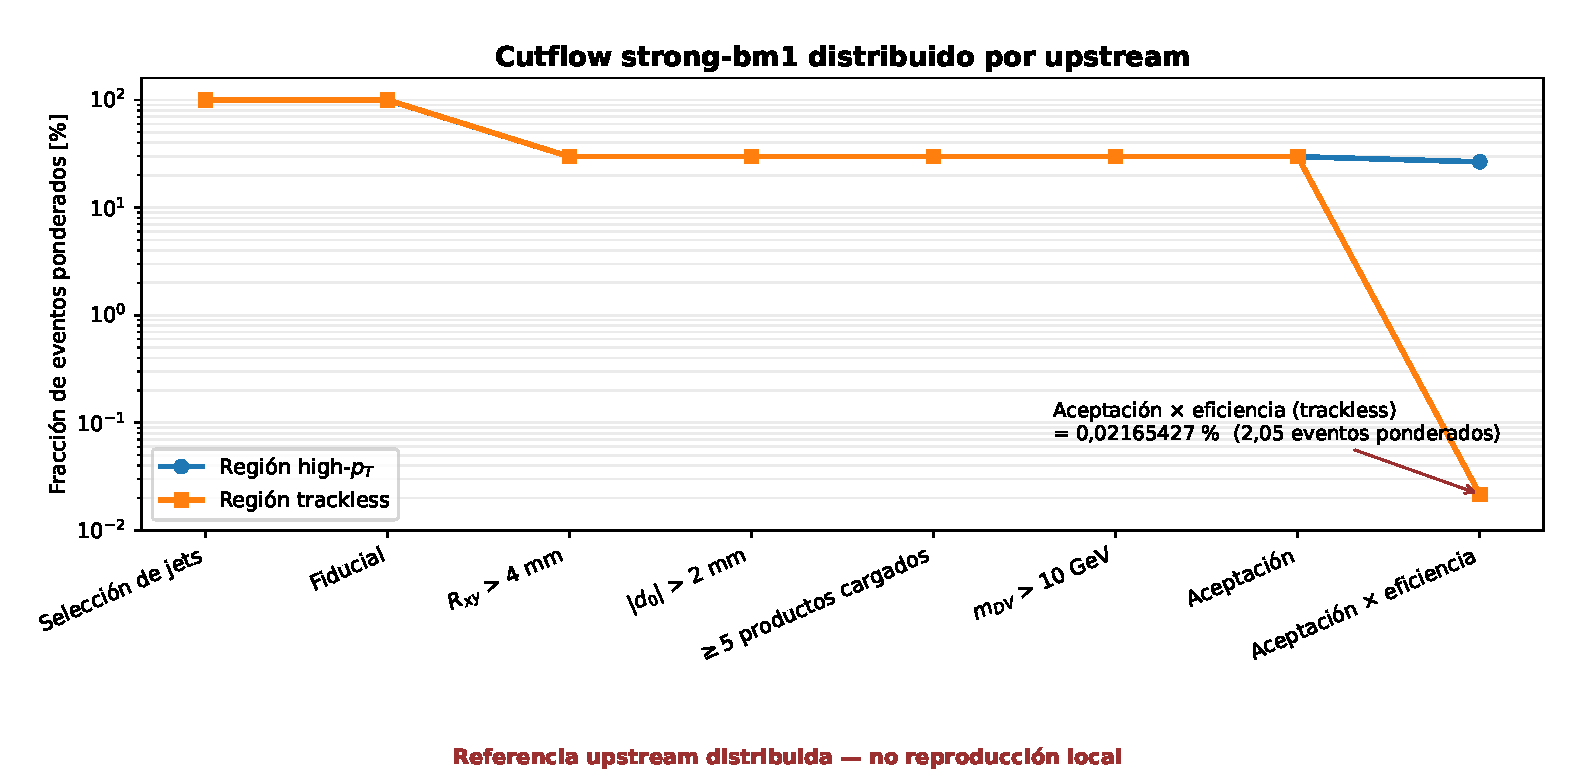
\includegraphics[width=0.98\textwidth,height=0.76\textheight,keepaspectratio]{reference_cutflow_upstream.pdf}

  \vspace{0.1em}
  {\small Gate B exige nuestros propios eventos, manifest y comparación explícita contra estas cifras.}
  \source{cutflow de referencia strong-bm1 (\texttt{gluino\_run01})}
\end{frame}

\begin{frame}{Dónde aporta este recast a nuestro modelo}
  \vspace{0.3em}
  \begin{tabular}{lccc}
    \toprule
    Canal de $S$ & Actividad hadrónica & DV multitrack & Utilidad\\
    \midrule
    $b\bar b$ & alta & sí & \textbf{HIGH}\\
    $gg$ & alta tras hadronización & sí & \textbf{HIGH}\\
    $WW/ZZ$ hadrónico & alta & sí & \textbf{HIGH}\\
    $Z\gamma$, con $Z$ hadrónico & media & condicional & \textbf{MEDIUM}\\
    $\gamma\gamma$ & baja & no natural & \textbf{LOW}\\
    \bottomrule
  \end{tabular}
  \vspace{0.9em}

  $\gamma\gamma$ no es una firma primaria aquí: dos fotones no dan los tracks cargados
  que el DV necesita. Esta utilidad es potencial: todavía no es eficiencia validada.
  \source{canales de decaimiento de scalar-recast-v0}
\end{frame}

\begin{frame}{Cuatro diferencias que debemos controlar}
  \begin{itemize}
    \item \textbf{PDG hardcoded}: el código busca neutralinos 1000022/23/24;
          hay que parametrizar la identidad del LLP para ver a $S$.
    \item \textbf{Algoritmo de jets}: el paper describe anti-$k_t$ $R=0.4$;
          el código usa $k_t$ $R=0.4$.
    \item \textbf{Fotones}: entran a FastJet sin aislamiento dedicado y pueden
          agruparse en jets.
    \item \textbf{Dominio de las eficiencias}: las parametrizaciones ATLAS son
          aproximadas y dependen de la topología SUSY que las originó.
  \end{itemize}
  \vspace{0.8em}
  \centering
  Cada cambio va detrás de una regresión: la línea base SUSY no debe moverse.
  \source{supuestos de scalar-recast-v0; \upcode}
\end{frame}

\begin{frame}{scalar-recast-v0: arquitectura lista, física pendiente}
  \begin{columns}[T]
    \column{0.48\textwidth}
    \textbf{Ya define}
    \begin{itemize}
      \item la arquitectura $gg\to h^*\to SS$;
      \item la relación $\Gamma=\hbar/\tau$;
      \item formatos, contratos y utilidad por canal.
    \end{itemize}
    \vspace{0.5em}
    \textbf{Todavía sin fijar}
    \begin{itemize}
      \item UFO y acoplamientos;
      \item PDG, masa, anchura y vida media;
      \item tabla completa de BR y merging.
    \end{itemize}
    \column{0.48\textwidth}
    \textbf{Es una arquitectura reconstruida, no una card física}: organiza
    nuestros supuestos y templates; no recupera la card original ni autoriza
    generación.
    \vspace{0.7em}

    \centering\texttt{RECONSTRUCTED}\\[0.2em]
    \texttt{generación NOT\_RUN}\\[0.2em]
    \texttt{validación física NOT\_RUN}
  \end{columns}
  \source{contrato físico de scalar-recast-v0}
\end{frame}

\begin{frame}{Dónde encaja este recast en el proyecto}
  \vspace{0.2em}
  \centering
  \begin{tabular}{@{}c@{\hspace{1.4em}}l@{}}
    \fbox{\parbox{0.30\textwidth}{\centering escaneos y puntos físicos\\{\small 2HDM: masa, anchura, $c\tau$, BR}}}
      & {\small\texttt{dihiggs} $+$ \texttt{dihiggs\_boundary}}\\[0.3em]
    $\downarrow$ & {\footnotesize\color{gray}punto validado por teoría y HiggsBounds/HiggsSignals}\\[0.3em]
    \fbox{\parbox{0.30\textwidth}{\centering producción y secciones eficaces\\{\small MadGraph, UFO, $\sigma$}}}
      & {\small\texttt{dihiggs\_hep\_cross}}\\[0.3em]
    $\downarrow$ & {\footnotesize\color{gray}eventos y $\sigma$, bajo un contrato de punto de modelo}\\[0.3em]
    \fbox{\parbox{0.30\textwidth}{\centering\textbf{aceptación $\times$ eficiencia}\\{\small recast DV+jets}}}
      & {\small\textbf{\texttt{dihiggs\_llp\_recast} --- este repo}}\\[0.3em]
    $\downarrow$ & {\footnotesize\color{gray}cutflows y manifests}\\[0.3em]
    \fbox{\parbox{0.30\textwidth}{\centering resultados y paper}} & {\small\texttt{paper}}\\
  \end{tabular}
  \vspace{0.8em}

  \raggedright\small
  Este repo recibe un punto físico y sus eventos, y devuelve cutflows para la
  reinterpretación. No explora el espacio 2HDM, no sustituye la producción MadGraph
  y no es el repositorio del artículo.
  \source{mapa del proyecto en \texttt{paper}; contrato punto de modelo $\to$ recast en \texttt{hep\_cross}}
\end{frame}

\begin{frame}{Tres decisiones y el próximo resultado comprobable}
  \textbf{Lo que necesitamos decidir hoy}
  \begin{enumerate}
    \item Qué UFO y qué tratamiento de $gg\to h^*\to SS$ aprobamos.
    \item Qué PDG, masa, vida media/anchura y tabla completa de BR definen
          el primer punto.
    \item Qué criterio exacto de Gate B habilita la parametrización escalar.
  \end{enumerate}
  \vspace{0.7em}
  \textbf{Gate técnico inmediato}: recuperar $\langle L_{3D}\rangle\approx 8.8$ mm en el
  toy $m=250$ GeV, $c\tau=5.1$ mm. Sólo entonces comparamos el cutflow DV A/B.
  \vspace{0.5em}
  \textbf{Próximo resultado comprobable}: un Gate B documentado sobre strong-bm1.
  Después parametrizamos sólo el PDG y el modo de análisis, y exigimos que la
  línea base SUSY siga dando el mismo cutflow antes del primer smoke escalar.
  \source{plan de reproducción; contrato de validación; scalar-recast-v0; Mission 01 execution report}
\end{frame}

\end{document}
